\documentclass[11pt,a4paper]{article}

\usepackage[margin=2cm]{geometry}
\usepackage{amsmath,amssymb}
\usepackage{graphicx}
\usepackage{booktabs}
\usepackage{tabularx}
\usepackage{caption}
\usepackage{float}
\usepackage{enumitem}
\usepackage{xcolor}
\usepackage{array}
\usepackage[colorlinks=true,linkcolor=blue!50!black,citecolor=blue!50!black,urlcolor=blue!50!black]{hyperref}

\graphicspath{{figures/}}
\captionsetup{font=small,labelfont=bf,skip=3pt}
\setlist{itemsep=1pt,topsep=2pt}
\setlength{\parskip}{3pt}
\setlength{\parindent}{0pt}
\newcommand{\todo}[1]{\textcolor{red}{[#1]}}
\newcolumntype{L}{>{\raggedright\arraybackslash}X}

\begin{document}

%=====================================================================
% Title block
\begin{center}
{\LARGE\bfseries Mangrove Maze}\\[3pt]
{\large Loops in the Indian Sundarbans tidal channel network, 2016--2026}\\[6pt]
ID5080 Complex Networks \quad$\cdot$\quad Project \todo{P0X} \quad$\cdot$\quad Team Mangrove Maze Runners\\[3pt]
\todo{Full name (roll number), one per member}\\[3pt]
November 2026 \quad$\cdot$\quad Code and data: \texttt{ID5080\_MangroveMazeRunners\_code.zip}
\end{center}

%=====================================================================
\section{What network did you build}

A \textbf{node} is a junction where tidal channels meet, or a channel end: an \emph{inlet} where a channel leaves the image on the land side, or an \emph{outlet} where it reaches the sea. An \textbf{edge} is one channel segment between two such points; in the real world it is a stretch of water that boats, water, sediment and salt can travel along. Edges carry the channel's mean width and centreline length. The graph is \textbf{undirected}, and allows parallel edges (two channels around one island). Planarity follows from the construction: channels in an image cannot cross without meeting at a junction.

\textbf{Alternatives considered and rejected.}
\begin{itemize}
  \item \emph{A directed graph}, as RivGraph builds for rivers \cite{rivgraph_esurf}. Tides reverse the flow twice a day, and RivGraph's direction rules produced directed cycles in 2016, 2024 and 2025. Where a direction was needed (inlet-to-sea paths), we oriented each edge towards the sea by graph distance instead.
  \item \emph{The full tidal network with every dead-end creek.} On a January 2016 test image this graph split into 63 components, because narrow creeks break up at 30 m. We kept only the system connected to inlets and the sea.
  \item \emph{The raw RivGraph skeleton} (1,453 nodes in 2022). Most of its nodes are spurs and pass-through points, not junctions.
  \item \emph{Width-weighted edges for all measures.} Width is uncertain at 30 m and estuary links are kilometres wide, so topology measures use unweighted edges; widths are used only for the conductance analysis.
  \item \emph{Separate outlets vs one sea node.} We keep separate outlets in the stored graphs, and join them to one sea node when computing paths to the sea and connectivity, because all outlets open onto the same Bay of Bengal.
\end{itemize}

%=====================================================================
\section{Where the data came from}

All images come from the \textbf{Copernicus Browser} (\url{https://browser.dataspace.copernicus.eu}), Sentinel-2 Level-\todo{2A/1C} scenes, exported with the browser's \textbf{NDWI visualisation} as 8-bit RGB GeoTIFFs (UTM zone 45N, EPSG:32645), 2500 $\times$ 1925 px at about 30.2 $\times$ 30.5 m per pixel. NDWI $= (\text{Green} - \text{NIR})/(\text{Green} + \text{NIR})$ \cite{mcfeeters1996}; the visualisation colours water blue and land green. One scene per year was chosen between mid-October and mid-November, on the clearest available day:
17 Oct 2016, 17 Oct 2017, 16 Nov 2019, 15 Nov 2020, 10 Nov 2021, 21 Oct 2022, 16 Oct 2023, 14 Nov 2024, 22 Oct 2025, 20 Oct 2026. No usable 2018 scene was found \todo{reason}. The view was centred on the Indian Sundarbans; the overlap of all ten scenes is 21.53--22.04$^\circ$N, 88.47--89.18$^\circ$E. A separate scene of 18 Jan 2016 was used only for early testing.
Files were downloaded on or before 27 October 2026 (file dates) \todo{exact access dates and export settings: zoom level, resolution option}. Copernicus Sentinel data are free and open; no other permission was needed.

%=====================================================================
\section{From raw data to a network}

The pipeline is in \texttt{common/sundarbans\_rg.py} (functions named below) and is run for all years by \texttt{scripts/01\_build\_graphs\_and\_metrics.py}.
\begin{enumerate}
  \item \textbf{Common grid} (\texttt{common\_grid}, \texttt{read\_rgb}). Scenes shift by up to 3 km, so all are resampled (nearest neighbour) onto their overlap, 2414 $\times$ 1830 px (72.9 $\times$ 55.7 km).
  \item \textbf{Water mask} (\texttt{water\_mask}). A pixel is water if blue $>$ green in the NDWI visualisation. Water objects and holes under 30 px are removed.
  \item \textbf{Shoreline} (\texttt{closed\_land}, \texttt{common\_shoreline}). The land mask is closed with an 80 px ($\approx$2.4 km) disc, at quarter resolution, to bridge river mouths; its boundary is the shoreline. One shoreline is used for all years, from pixels that are water in at least 5 of the 10 images.
  \item \textbf{Skeleton and raw network}: RivGraph \cite{rivgraph_joss} \texttt{skeletonize} and \texttt{compute\_network}.
  \item \textbf{Inlets} (\texttt{write\_inlets}): degree-1 nodes within 2 px of the top, left or right edge, on the land side.
  \item \textbf{Pruning} (\texttt{prune\_sundarbans}): remove spurs, cut links at the shoreline (cut ends become outlets), remove disconnected pieces and one-pixel links, and merge degree-2 nodes. RivGraph's own \texttt{prune\_network} crashes when the shoreline splits the scene into several estuary systems, so each inlet's system is pruned and the largest is kept.
  \item \textbf{Graphs} (\texttt{to\_graphs}): NetworkX multigraphs G1--G10, saved as GraphML and a pickle.
\end{enumerate}
Discarded: everything seaward of the shoreline, all components other than the main system, and dead-end creeks other than inlets and outlets. Degree-4 nodes are not split; 0--2 remain per year.

\textbf{Judgement calls.} Water rule blue $>$ green (a per-image Otsu threshold \cite{otsu1979}, tried first, can shift between years); 30 px minimum object; 80 px closing disc; 5-of-10 vote for the shoreline; 2 px edge band for inlets; the largest estuary system only; resolution 30 m as exported.

\begin{figure}[t]
\centering
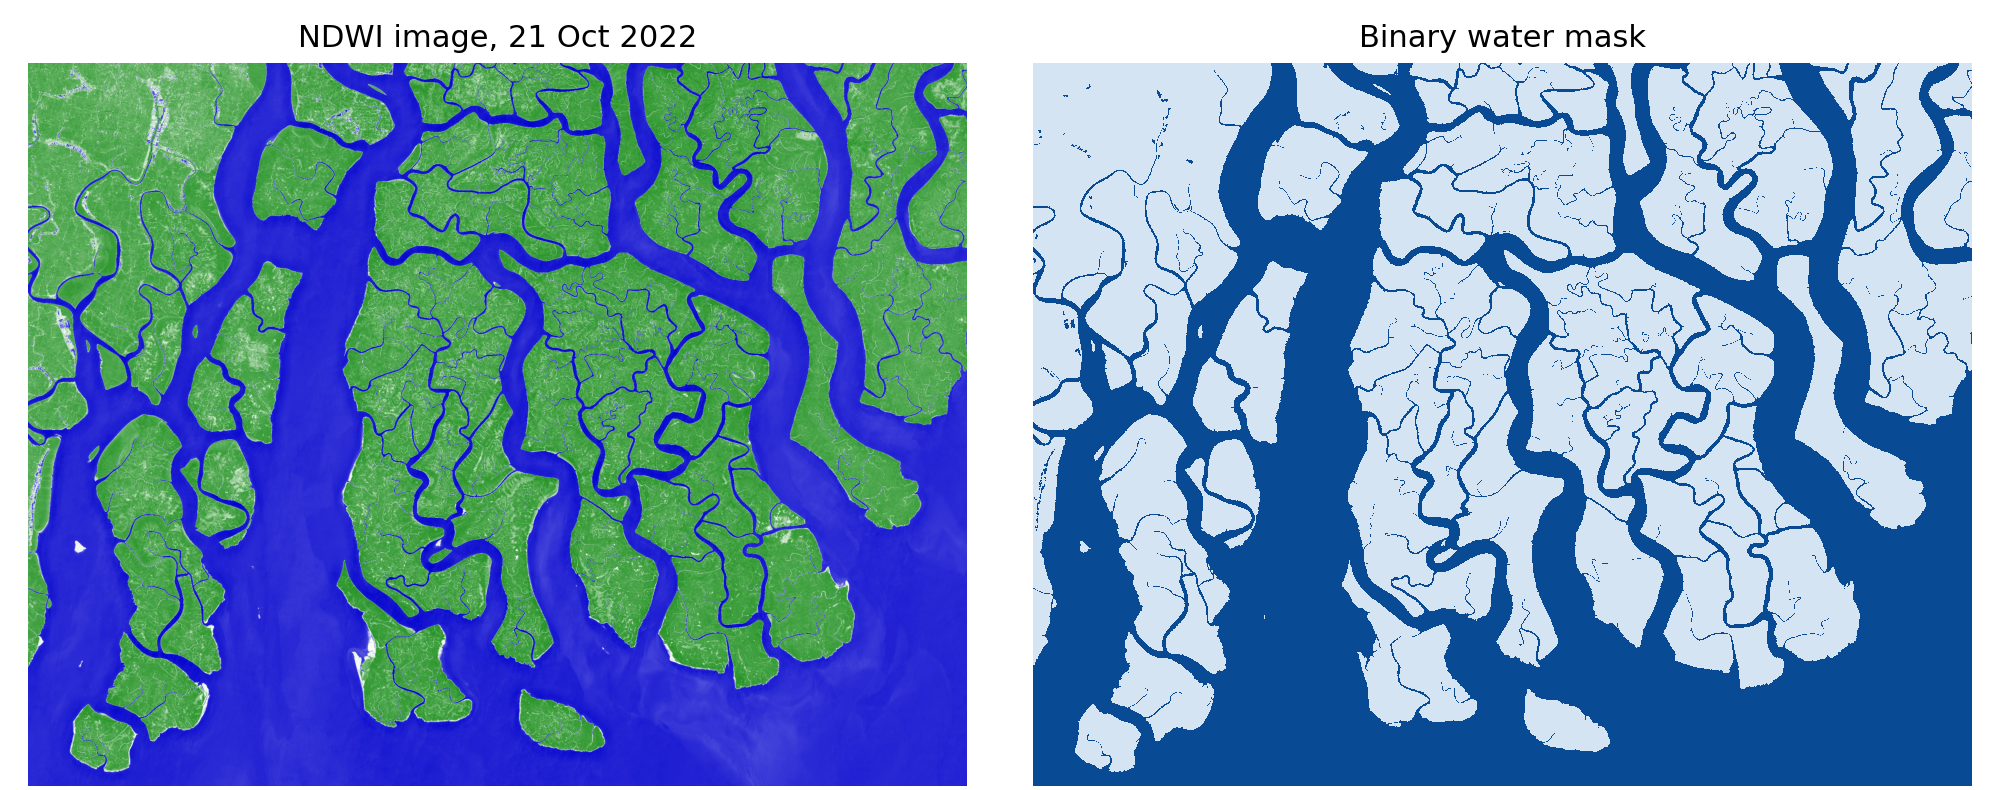
\includegraphics[width=0.40\textwidth]{image_and_mask.png}\hfill
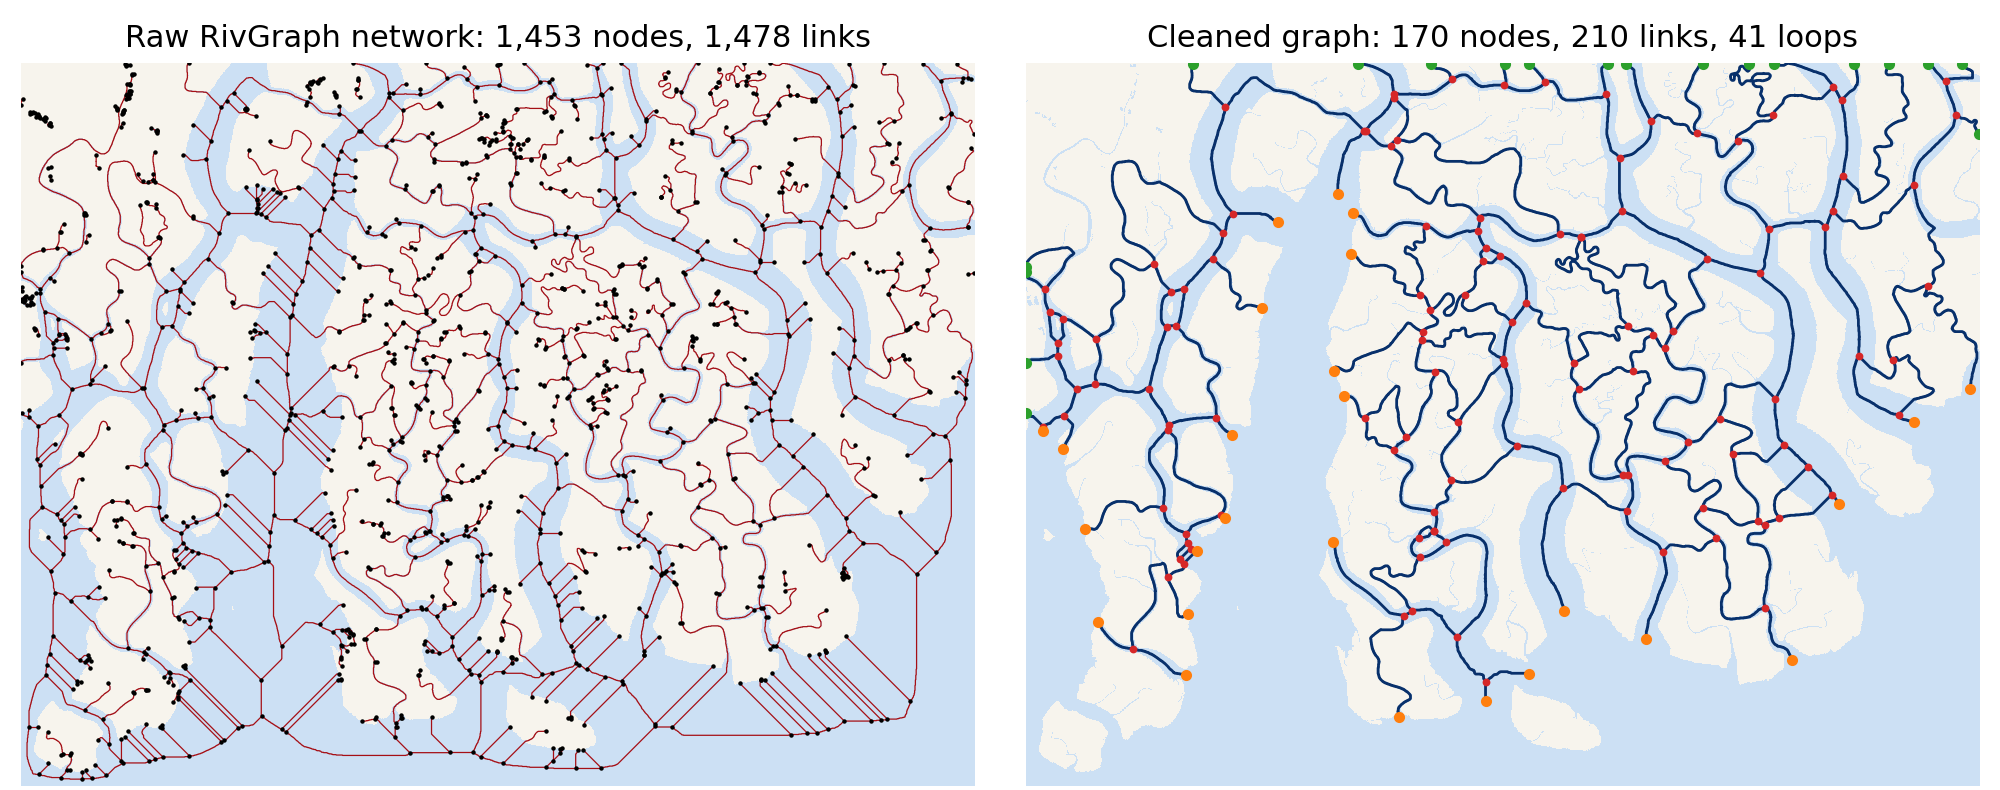
\includegraphics[width=0.58\textwidth]{raw_vs_clean.png}
\caption{2022: NDWI image and water mask; raw RivGraph network (1,453 nodes) and the cleaned graph (170 nodes, 210 edges, 41 loops).}
\end{figure}

%=====================================================================
\section{What is in the data folder}

Paths are relative to the top of the code folder (Table~\ref{tab:files}); \texttt{README.md} gives the run order and \texttt{MANIFEST.md} lists every file. \path{scripts/01}--\path{04} are \path{01_build_graphs_and_metrics.py}, \path{02_basic_properties.py}, \path{03_simplified_weighted_graphs.py} and \path{04_final_figure.py}.

\begin{table}[H]
\centering\footnotesize
\begin{tabularx}{\textwidth}{@{}p{5.0cm}Lrp{3.6cm}@{}}
\toprule
File & What it holds & Size & Produced / used by \\
\midrule
\path{data_raw/images/*.tiff} (10) & Raw Copernicus NDWI GeoTIFFs, one per year & 60 MB & Downloaded; read by \path{scripts/01} \\
\path{data_processed/timeseries/}\newline\path{shoreline_common.gpkg} & The shared shoreline & 144 kB & \path{scripts/01} \\
\path{data_processed/timeseries/<date>/} & Water mask, inlets and RivGraph network per year & 0.8 MB/year & \path{scripts/01} \\
\path{data_processed/timeseries/graphs/}\newline\path{G{k}_<date>.graphml}, \path{B{k}_<date>.graphml} & Cleaned graphs G1--G10; one random tree per year & 0.9 MB & \path{scripts/01} \\
\path{data_processed/timeseries/graphs/}\newline\path{all_graphs.pkl}, \path{index.csv} & All graphs with inlets/outlets; graph--date--file index & 1.9 MB & \path{scripts/01} \\
\path{data_processed/timeseries/}\newline\path{metrics_G.csv} & Parameters of G1--G10 (Sec.~7) & 3 kB & \path{scripts/01} \\
\path{data_processed/timeseries/}\newline\path{metrics_baseline_samples.csv} & Parameters of 1,000 random trees per year; the first 10 are used & 2.0 MB & \path{scripts/01} \\
\path{data_processed/timeseries/}\newline\path{trend_tests.csv}, \path{zscores_vs_baseline.csv} & Kendall's $\tau$ and distances from the trees & 2 kB & \path{scripts/01} \\
\path{data_processed/basic_properties/*.csv} & Section 5 properties, ER samples, top betweenness & 188 kB & \path{scripts/02} \\
\path{data_processed/timeseries_weighted/} & Weighted, simplified graphs and their parameters (Sec.~6) & 15 MB & \path{scripts/03} \\
\path{figure/ID5080_MangroveMazeRunners_fig.pdf} & Final network figure & 0.2 MB & \path{scripts/04} \\
\path{members/mohd_hamza/}\newline\path{temporal_analysis/} & Figure~2 and the five-parameter trend tests & 0.1 MB & \path{make_temporal_figures.py} \\
\path{members/mohd_hamza/dip_2023_2024/}\newline\path{sensitivity.csv} & Loops and bridges under other water rules (Sec.~6) & 5 kB & \path{dip2.py} \\
\todo{conductance, connectivity, persistence files} & Section 7 results from other members & & \todo{member scripts} \\
\bottomrule
\end{tabularx}
\caption{Data files.}\label{tab:files}
\end{table}

%=====================================================================
\section{Basic network properties}

Parallel edges were merged (0--7 per year) to compute these on simple graphs. The comparison uses 100 Erdős–Rényi graphs with the same $n$ and $m$ per year (values are means).

\begin{table}[H]
\centering\small
\begin{tabular}{@{}p{5.2cm}cc@{}}
\toprule
 & G1--G10 (range) & Erdős–Rényi $G(n,m)$ \cite{er1959} \\
\midrule
Nodes $n$ / edges $m$ & 139--172 / 169--211 & same \\
Density & 0.014--0.018 & same \\
Mean degree & 2.39--2.46 & same \\
Share of nodes with degree 1 / 3 / other & 24--30 / 67--72 / $\le$9\% & 21 / 21 / 57\% \\
Components / largest & 1 / all nodes & 14--17 / 87--92\% of nodes \\
Mean shortest path (hops) & 11.6--13.4 & 5.2--5.4 \\
Diameter (hops) & 31--36 & 12--13 \\
Clustering (average) & 0.030--0.058 & 0.009--0.013 \\
Independent loops & 29--40 & 43--56 \\
Planar & all & none \\
\bottomrule
\end{tabular}
\end{table}

Against a random graph of the same size, the delta network is \emph{connected, planar and long}: random wiring makes shortcuts across the whole area (mean path 5 hops), while real channels only join neighbours, so paths are more than twice as long. Degrees are almost only 1 and 3, because channels split one into two; random graphs have a broad Poisson spread. Clustering is low in both, but higher in the delta, from small triangles where channels meet close together.

\textbf{Centrality.} The node with the highest betweenness lies at about 21.99$^\circ$N, 88.73$^\circ$E \todo{name the river/junction}, on a channel about 3.4 km wide. It is the top node in 8 of the 10 years (betweenness 0.41--0.47). This is plausible: it joins several wide channels near the middle of the network's northern part, so many shortest paths cross it.

%=====================================================================
\section{Turning the knob}

\textbf{Water threshold.} Rerunning all years with other blue--green cut-offs (\texttt{sensitivity.csv}):

\begin{table}[H]
\centering\footnotesize
\begin{tabular}{@{}lcccccccccc@{}}
\toprule
Loops & 2016 & 2017 & 2019 & 2020 & 2021 & 2022 & 2023 & 2024 & 2025 & 2026 \\
\midrule
blue $-$ green $> +15$ & 35 & 42 & 41 & 41 & 39 & 41 & 31 & 31 & 40 & 41 \\
$> 0$ (used) & 35 & 42 & 41 & 41 & 39 & 41 & 31 & 31 & 40 & 41 \\
$> -15$ & 45 & 45 & 42 & 41 & -- & 42 & 41 & 38 & 44 & 41 \\
$> -30$ & 50 & -- & 48 & 48 & 45 & 44 & 49 & 48 & 48 & 44 \\
$> 0$ + close 1 px gaps & 41 & 45 & 42 & 43 & 42 & 44 & 33 & 32 & 43 & 45 \\
\bottomrule
\end{tabular}
\caption{Independent loops under other water rules. -- = RivGraph failed for that run.}
\end{table}

\textbf{Held up:} raising the threshold changes nothing (water and land are well separated), the network stays loop-rich (31--50 loops) and far from a tree under every rule, and bridge share stays 0.28--0.37. \textbf{Moved:} lower thresholds join narrow creeks and add loops, and the 2023--24 dip (31 loops) disappears at $-15$ (41 and 38). So the absolute loop count depends on the threshold, and the 2023--24 dip is a detection effect rather than a physical change.

\textbf{Baseline sampling.} With 1,000 random trees per year instead of 10, the distances from the trees change (e.g.\ $\lambda_2$: $+4.8$ to $+8.0$ sd instead of $+4.7$ to $+11.1$), but every conclusion is the same.

\textbf{Graph simplification.} Contracting short, wide links (\path{common/sundarbans_simplified_network.py}, \path{scripts/03}) removes 7 nodes per year; loops and bridge share are unchanged, and mean inlet-to-sea path drops from 5.9 to 5.4 links.

\textbf{Resolution.} Not tested: all images are 30 m. Repeating at 10 m and 90 m is the main missing experiment.

%=====================================================================
\section{Our question: how far is the delta from a tree, and does it change?}

\textbf{Against random trees.} For each year we built 10 random trees on the same nodes (outlets as roots, inlets as leaves, junctions with random parents, seeds fixed) in \texttt{tree\_nulls.py}, and compared five parameters, with outlets joined to one sea node.

\begin{figure}[H]
\centering
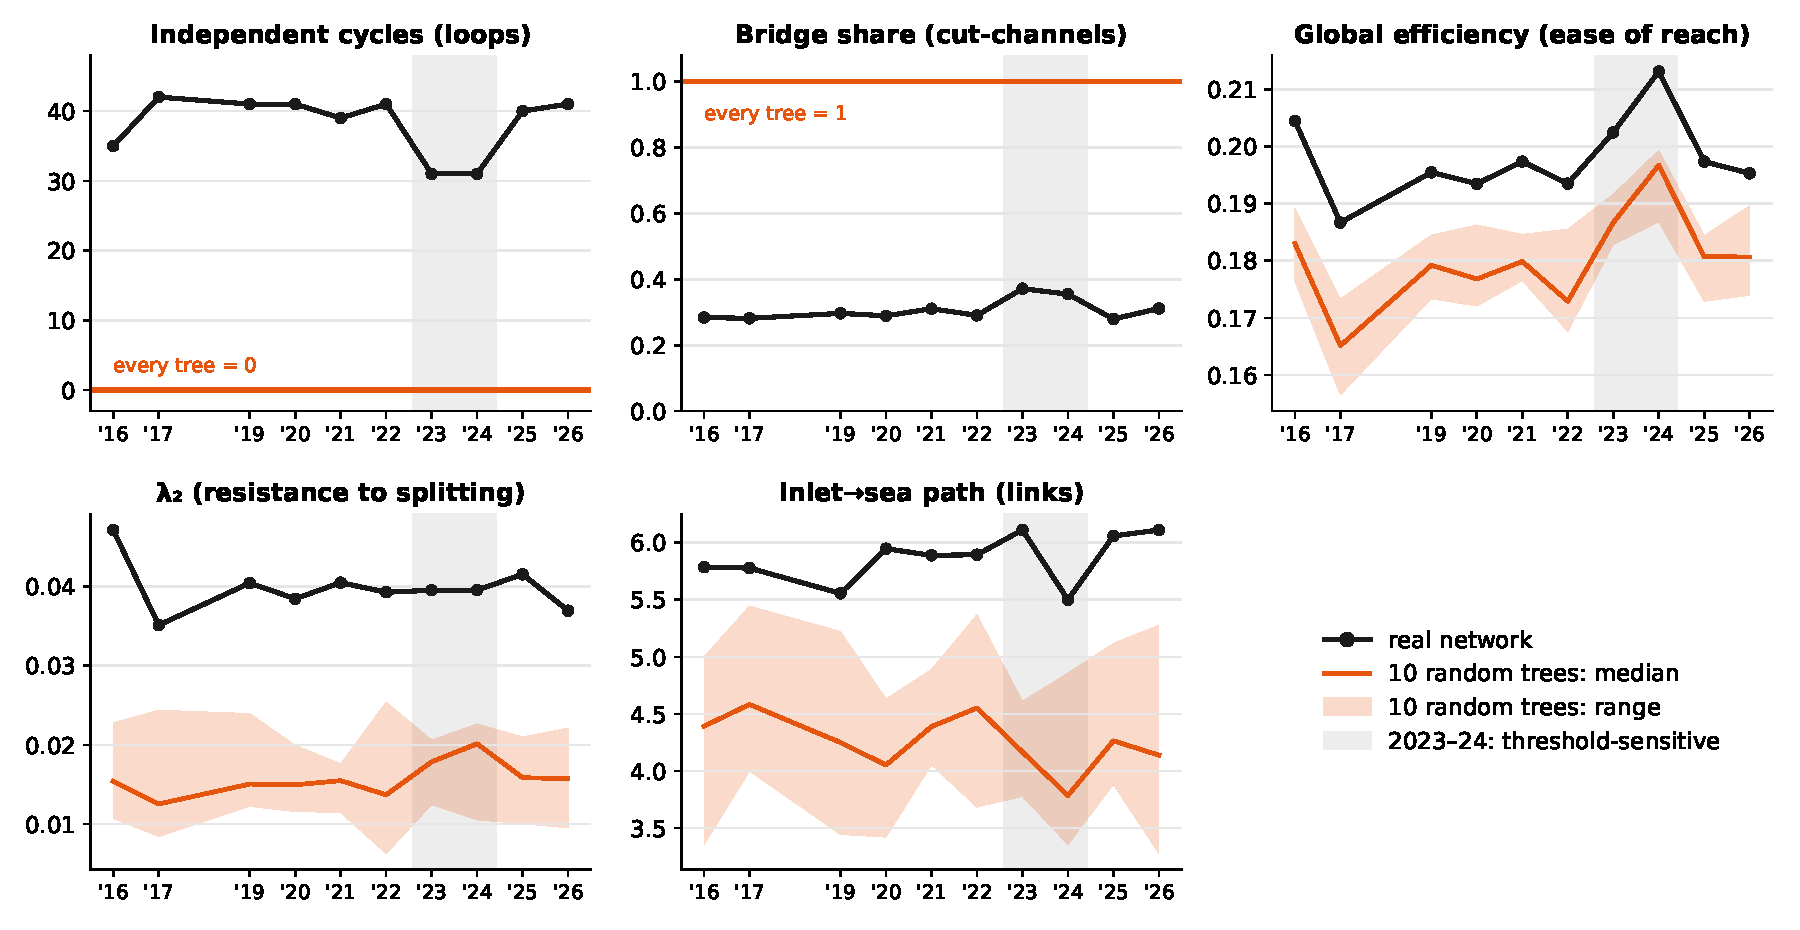
\includegraphics[width=0.78\textwidth]{comparison_5.pdf}
\caption{Real network (black) against the median and range of 10 random trees per year (orange), 2016--2026.}
\end{figure}

The delta has 31--42 loops a year where trees have none, and only 28--37\% of its channels are bridges, against 100\%. Global efficiency (0.19--0.21) and algebraic connectivity $\lambda_2$ (0.035--0.047) exceed all 10 trees in every year. Inlet-to-sea paths are longer (5.5--6.1 links against a tree median of 3.8--4.6). No parameter has a significant trend (Kendall's $\tau$, all $p > 0.1$).

\textbf{Connectivity} \todo{member}. With all outlets merged into one sea node, the giant component holds every node every year, and the loop-connected core (dead ends removed) holds 82--88\% of nodes and every loop. The cycle rank rises from 57 (2024) to 66 (2025) and 69 (2026), after cyclones Remal and Dana; given the threshold sensitivity above, this is a hypothesis only.

\textbf{Electrical network} \todo{member}. With conductance $g_{ij} = \bar w_{ij}/\ell_{ij}$, inlets at $V=1$ and outlets at $V=0$, we solved $LV = I_{\text{ext}}$ for the effective conductance $G$. The topological conductance $G_{\text{topo}}$ (all $g_{ij} = 1$) stays at 1.90--2.18, and the geometric effect $\eta = G/(\bar g\,G_{\text{topo}})$ averages 1.08 but fluctuates between 0.91 and 1.29. Comparing 2024 ($\eta \approx 0.92$) with 2025 ($\eta \approx 1.29$), edge conductances and main current paths are almost the same; the difference is extra low-conductance parallel routes.

\begin{figure}[H]
\centering
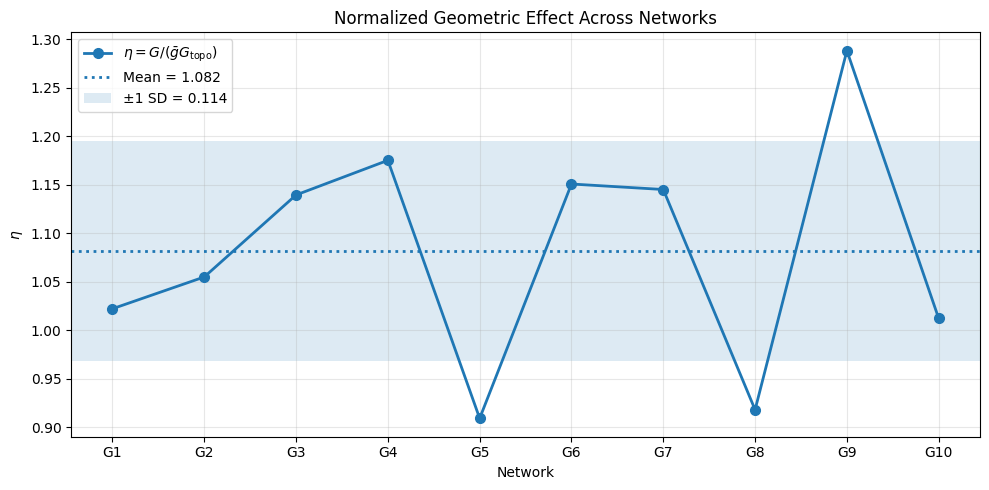
\includegraphics[width=0.37\textwidth]{eta.png}\hfill
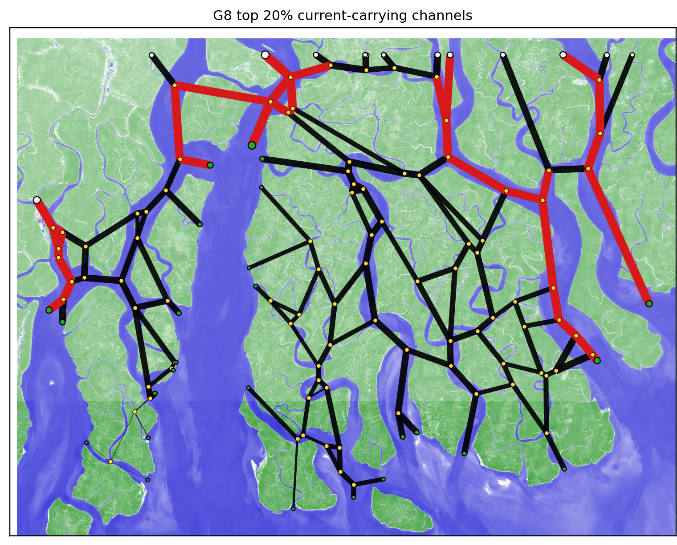
\includegraphics[width=0.30\textwidth]{G8_current.png}\hfill
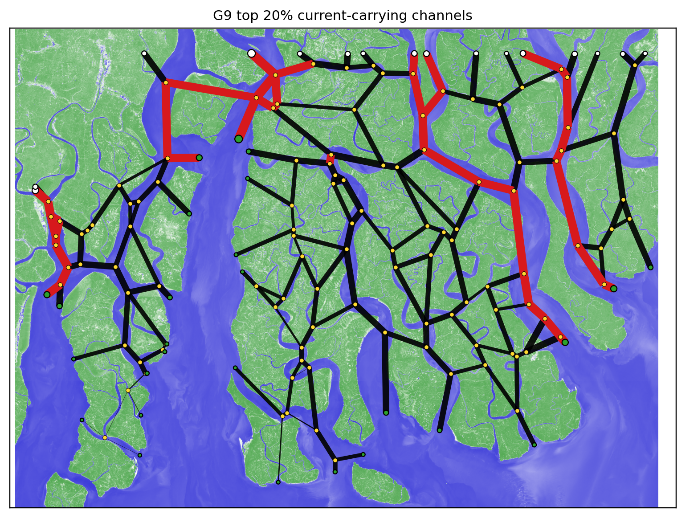
\includegraphics[width=0.30\textwidth]{G9_current.png}
\caption{$\eta$ per network (left), and the 20\% of channels carrying the most current (red) in 2024 and 2025.}
\end{figure}

\textbf{Persistence} \todo{member}. Overlaying channel skeletons from all snapshots, 66\% of channel length (722 of 1,099 km) is present in all ten; wide channels persist and change is in narrow creeks. On a 4 $\times$ 4 grid of tiles, loops are concentrated inland (meshedness up to 0.11), while seaward tiles are tree-like (no loops, bridge share 1).

\begin{figure}[H]
\centering
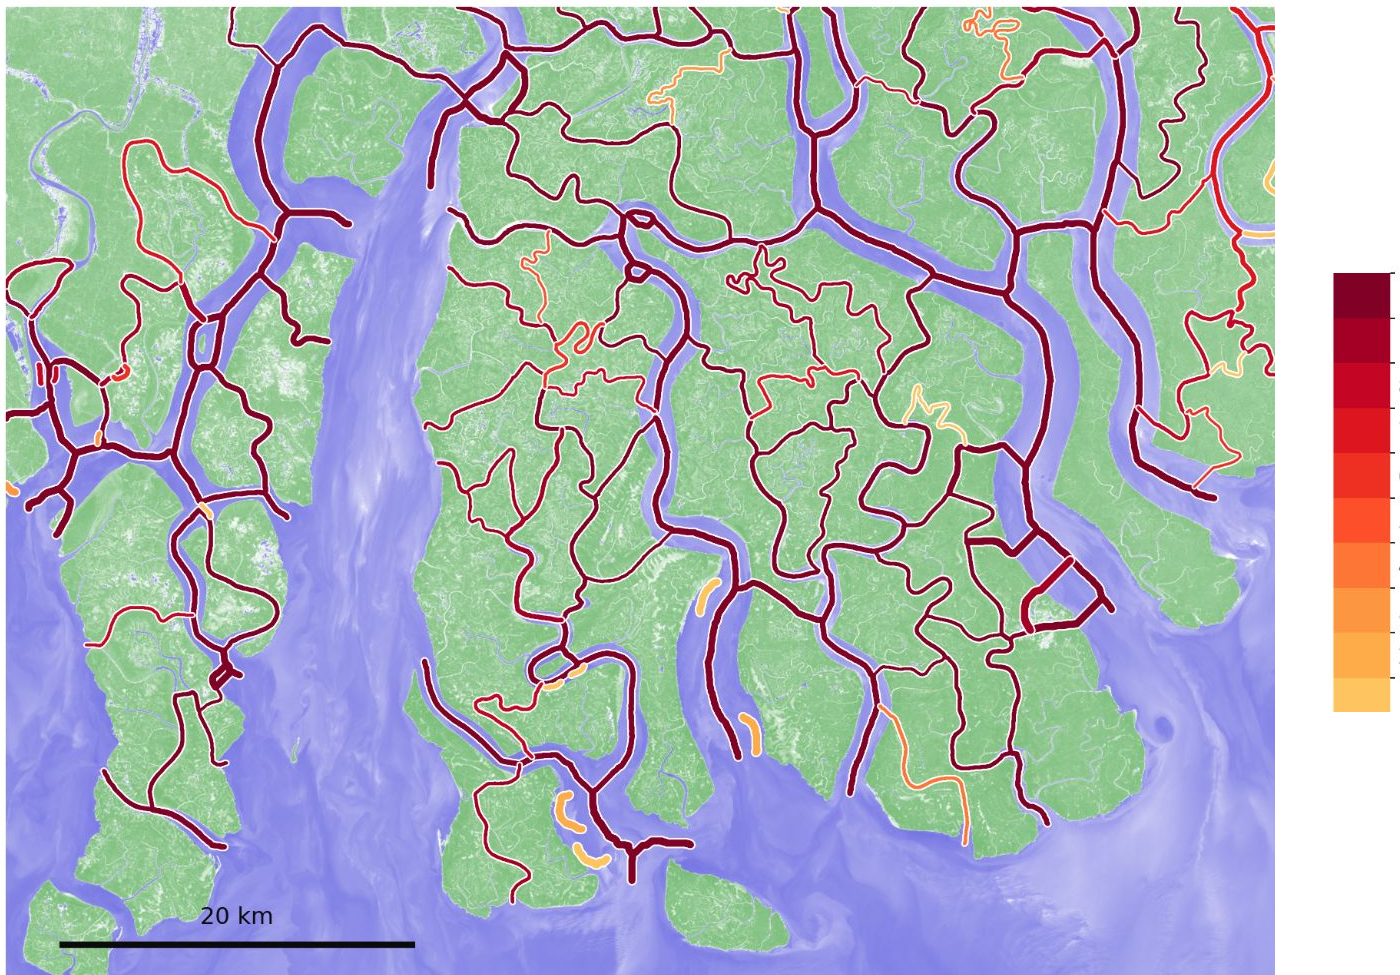
\includegraphics[width=0.44\textwidth]{persistence_map_crop.png}\hfill
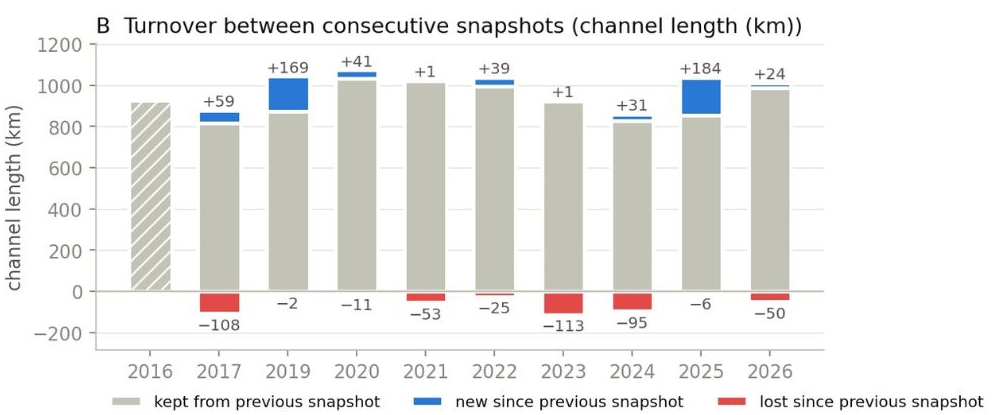
\includegraphics[width=0.53\textwidth]{turnover.png}
\caption{Channels coloured by the number of the 10 snapshots containing them (light: 1, dark: 10), and channel length kept, gained and lost between snapshots.}
\end{figure}

\textbf{Final figure} (\texttt{ID5080\_MangroveMazeRunners\_fig.pdf}). The 2022 channel network over its water mask, with channels that lie on a loop in blue and bridges in orange: only 29\% of channels are bridges, whereas in a tree every channel would be one.

\textbf{Answer.} The Sundarbans tidal network is planar, loop-rich and far from a tree in every year from 2016 to 2026, with no significant trend. Redundant parallel channels, more than the main channels, control how easily water moves through it.

%=====================================================================
\section{Difficulties, dead ends and limits}
\begin{itemize}
  \item \textbf{RivGraph pruning crashed} on our scenes, because the shoreline splits them into several estuary systems; we rewrote the step to prune each system and keep the largest. Its shoreline clipping also crashed on a zero-length intersection in the 2019 image, fixed by moving the shoreline by a fraction of a pixel.
  \item \textbf{RivGraph flow directions} contained cycles in three years and do not suit tides, so we dropped them (Section 1).
  \item \textbf{Per-image Otsu thresholds} were dropped for a fixed rule, so that thresholds could not shift between years.
  \item \textbf{The 2023--24 dip.} We first looked for a flood or cyclone cause in news and weather records; nothing fitted the timing or the 2025 recovery. Tests then showed it is threshold-sensitive, the missing channels are $\approx$92\% water in the masks, and both images have a paler band of land in the north, likely an image-processing difference.
  \item \textbf{Full tidal network with dead ends} broke into 63 components at 30 m; we used the connected system only.
  \item \textbf{Limits:} one image per year with uncontrolled tide stage; no 2018 image; 30 m only; dead-end creeks excluded; 10 random trees per year; conductance ignores depth and flow reversal; the connectivity figures include a 2018 snapshot not in our image set \todo{reconcile}; no ground-truth validation.
  \item \textbf{With another month:} several images per year at matched tide, 10 m resolution, Sentinel-1 radar for cloudy months, and a hand-digitised check of a few scenes.
\end{itemize}

%=====================================================================
\begin{thebibliography}{9}\small
\bibitem{tejedor2015} A.~Tejedor, A.~Longjas, I.~Zaliapin and E.~Foufoula-Georgiou. Delta channel networks: 2. Metrics of topologic and dynamic complexity for delta comparison, physical inference, and vulnerability assessment. \emph{Water Resources Research}, 51:4019--4045, 2015.
\bibitem{rivgraph_esurf} J.~Schwenk, A.~Piliouras and J.~C.~Rowland. Determining flow directions in river channel networks using planform morphology and topology. \emph{Earth Surface Dynamics}, 8:87--102, 2020.
\bibitem{rivgraph_joss} J.~Schwenk and J.~Hariharan. RivGraph: Automatic extraction and analysis of river and delta channel network topology. \emph{Journal of Open Source Software}, 6(59):2952, 2021.
\bibitem{mcfeeters1996} S.~K.~McFeeters. The use of the Normalized Difference Water Index (NDWI) in the delineation of open water features. \emph{International Journal of Remote Sensing}, 17(7):1425--1432, 1996.
\bibitem{otsu1979} N.~Otsu. A threshold selection method from gray-level histograms. \emph{IEEE Trans.\ Systems, Man, and Cybernetics}, 9(1):62--66, 1979.
\bibitem{er1959} P.~Erdős and A.~Rényi. On random graphs I. \emph{Publicationes Mathematicae}, 6:290--297, 1959.
\bibitem{tools} Software: Python, RivGraph, NetworkX, NumPy, SciPy, pandas, rasterio, GeoPandas, scikit-image, Matplotlib. Data: Copernicus Sentinel-2 via the Copernicus Browser.
\end{thebibliography}

%=====================================================================
\newpage
\section*{Signatures, contributions and AI use}

\emph{We confirm that the data in this report was collected by us as described, that we have not fabricated or altered any result, and that the contributions recorded below are accurate. We have declared our use of AI tools, and each of us can explain any part of this submission on request.}

\medskip
\begin{center}\footnotesize
\begin{tabularx}{\textwidth}{@{}p{2.4cm}p{1.8cm}Lp{3.4cm}p{2.4cm}@{}}
\toprule
Name & Roll no. & What I did & AI tools I used, and for what & Signature \& date \\
\midrule
Mohd Hamza & PH22B016 & Downloaded the 10 Sentinel-2 images (2016--2026) from the Copernicus Browser and ran the team's masking and graph pipeline on them to build G1--G10. Did the temporal analysis against the random-tree baseline (Sec.~7, Fig.~2; Kendall trend tests) and investigated the 2023--24 dip (Sec.~6, 8). Wrote this report. & Claude: help writing my analysis code, and formatting this PDF report. & \\[14pt]
\todo{Name} & \todo{Roll no.} & \todo{e.g.\ electrical-network conductance analysis} & \todo{} & \\[14pt]
\todo{Name} & \todo{Roll no.} & \todo{e.g.\ connectivity: GCC, GLCC, cycle rank} & \todo{} & \\[14pt]
\todo{Name} & \todo{Roll no.} & \todo{e.g.\ channel persistence and multiscale analysis} & \todo{} & \\[14pt]
\bottomrule
\end{tabularx}
\end{center}

\textbf{AI declaration.} Mohd Hamza used Claude (Anthropic) to help write the code for the temporal analysis and the 2023--24 checks, and to format this PDF report. \todo{Other members: tools and uses.} We checked the results by \todo{what you checked yourselves, e.g.\ inspecting every cleaned graph over its water mask, checking the loop formula by hand on G1, re-running the pipeline to get the same numbers}. \todo{Anything used but not fully understood.}

\end{document}
